% Auto-generated by scripts/build_ch5_evidence_tables.py (final drafting pass, 2026-10).
\begin{figure}[!htbp]
\centering
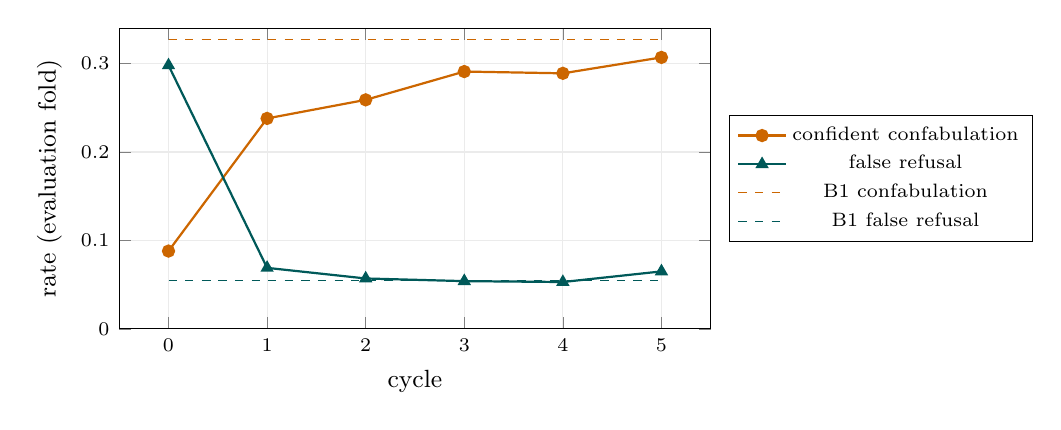
\begin{tikzpicture}
\begin{axis}[width=0.75\textwidth, height=5.4cm, xlabel={cycle}, ylabel={rate (evaluation fold)}, xtick={0,...,5},
  ymin=0, ymax=0.34, font=\small, tick label style={font=\scriptsize}, grid=major, grid style={black!8},
  legend style={font=\scriptsize, at={(1.03,0.5)}, anchor=west}]
  \addplot[orange!80!black, mark=*, thick] coordinates {(0,0.088) (1,0.238) (2,0.259) (3,0.291) (4,0.289) (5,0.307)};
  \addlegendentry{confident confabulation}
  \addplot[teal!70!black, mark=triangle*, thick] coordinates {(0,0.298) (1,0.069) (2,0.057) (3,0.054) (4,0.053) (5,0.065)};
  \addlegendentry{false refusal}
  \addplot[orange!80!black, dashed, domain=0:5] {0.327};
  \addlegendentry{B1 confabulation}
  \addplot[teal!70!black, dashed, domain=0:5] {0.055};
  \addlegendentry{B1 false refusal}
\end{axis}
\end{tikzpicture}
\caption[Confident confabulation against false refusal by cycle.]{Confident confabulation against false refusal by cycle. Both are defined through the verifier's own score, so they move in opposite directions as the refitted gate becomes more permissive.}
\label{fig:tradeoff}
\end{figure}
